\subsection{Convential Diagnosis Methods}
The most common conventional diagnosis method of detection involves
using ABCD rule which considers the Asymmetry, Border irregularity,
Colour irregularities and  Dermoscopic structures respectively of the
common pigmented skin lesions \citep{LOESCHER2013170}. 
The rule for classification was introduced in 1985 as abcd 
rule and was amended with abcde in 2004 where ‘E’ reflects the 
lesions which are evolving. An alternative method of examination of
pigmented skin lesions is  ugly duckling signs which was introduced 
to state the limitation of the ABCD rule \citep{DanielJensen2015}.
The ugly duckling signs state the spot which is unlike other 
lesions are great suspects of melanoma \citep{grob1998ugly}.
Despite the limitations of above methods, both provide a great
framework for clinicians and general audiences to spot melanoma 
based symptoms \citep{DanielJensen2015}.
Small malignant melanoma are millimeters in size in initial phases
of its growth.  
\\
\\
The micro-melanoma requires more attention to be
detected by physicians and researchers believe that small 
lesions possess challenges for medical professionals to 
clearly examine malignant based problems \citep{doi:10.1177/030089160409000125}.
Dermatoscopy is non-invasive microscopic imaging of pigmented skin 
lesions which provides clear imaging to perform proper analysis on 
pigmented skin lesions \citep{LOESCHER2013170}. 
The study was conducted in Italy for the period of five years in 
which ninety four melanoma based lesions. Furthermore, results 
were treated to examine the clinical and dermoscopic features of 
cutaneous melanoma lesions with maximum diameter of 3mm. 
The outcome of the research has shown that only samples of twenty two lesions which 
accounts for 2.4 percent of overall samples were decided based on
the clinical size feature of pigmented skin lesions \citep{doi:10.1177/030089160409000125}.
Moreover, the research mentions that dermoscopic results are more accurate to diagnose 
and has been an aid for early detection of melanoma skin cancer 
provided the clinicians are aware about disease \citep{doi:10.1177/030089160409000125}.
The result of dermatoscopic images is examined by dermatologists to classify the pigmented skin lesion.
Dermatologists select different approaches to examine pigmented
skin lesions which might include ABCDE rule or ugly duckling signs, 
where both the methods complement each other to detect pigmented skin lesions. 
The research proposed an addition of ‘F’ to mnemonic which uses both 
current methods ugly duckling sign and ABCDE rule which also account 
for funny or unlike lesions to be suspect of melanoma based lesion \citep{doi:10.1177/030089160409000125}.


\subsection{Functioning of Convolutional Neural Networks}
The convolutional neural networks are the feed-forwards neural 
networks which contains alternative convolutional layers and sampling 
layer which at the end is connected to fully connected neural networks \citep{liew2016gender}.
The objective of the convolutional layers is to extract the features from 
the given input image samples by applying filters which is used in the training 
of overall network.

\begin{figure}[!htp]
    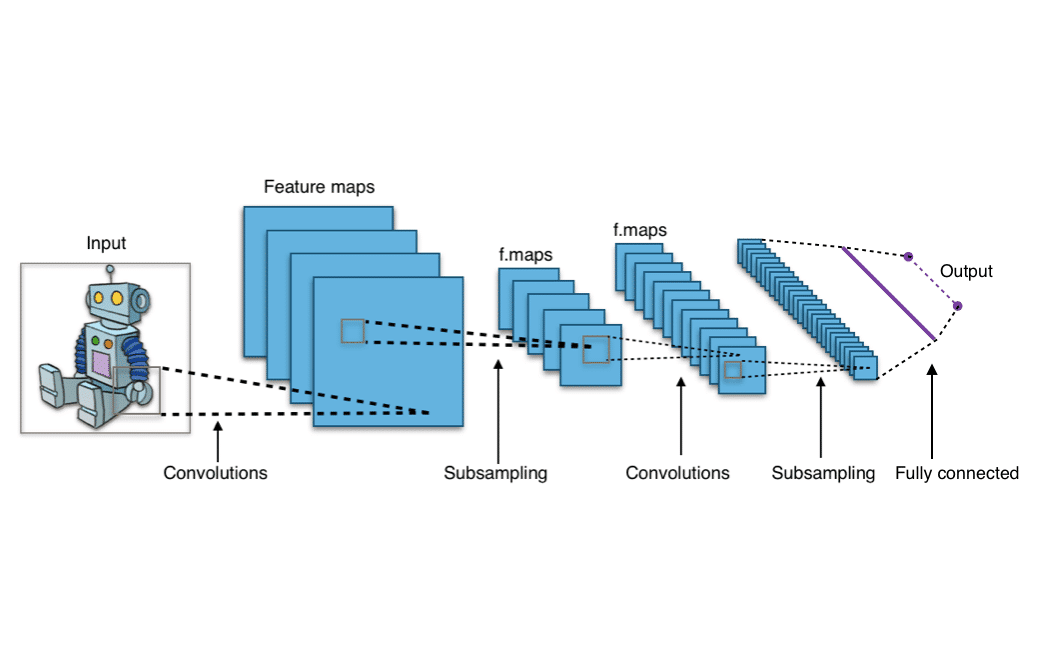
\includegraphics[width=\textwidth]{Images/cnn.png}
    \caption{Convolutional Neural Network}
    \label{figure:cnnf}
\end{figure}
The initial layer is known as the input layer in convolutional network 
which contains the pixel information of the image. The convolutional layer 
of the network determines the output of the neuron of perticular region 
by applying image kernels to extract the features from the images \citep{DBLP:journals/corr/OSheaN15}. 
The image kernels are the matrix of filter which are computed with the local region 
and produce the feature maps  \citep{DBLP:journals/corr/OSheaN15}. 
Furthermore as shown in \ref{figure:cnnf} sub sampling also 
known as downsampling is applied to the feature maps to reduce the dimensionality 
of the feature maps. In addition, there can exist various number of 
convolutional layers and sub sampling layer based on the architecture of the network.
The next layer in the network is flattening layer which reshapes the 
feature maps extract from previous convolutional layers of the network. 
At last the flattened information is passed to the fully connected neural network to analyse the relationships 
in the data and make appropriate predictions \citep{DBLP:journals/corr/OSheaN15}.  
\pagebreak

\subsection{SVM Algorithm to classify Pigmented Skin lesions}
Thompson Felsia and Jeyakumar proposed research in 2017 on 
support vector machine based classifier to detect multi-lesions skin cancer by analysing pigmented skin lesions with an accuracy of 86.37 percent.
The proposed investigation with SVM based classifier has performed image segmentation using SRM (support region merging) algorithm. Furthermore, it employs SURF (speed up robust features) to find the region 
of interest for feature extraction to get optimal classification performance based on vector-based technique \citep{thompson2017vector}. 
However, the research does not include image augmentation which generalises the predictions accurate to test in 
real-world environment. The research papers mention that support vector machine for automated classification of pigmented skin lesions is sensitive to the artefacts and can 
potentially increase the false positives which mean that predicted result for analysis was wrong positive prediction instead of an actual negative result. The investigation will perform image augmentation to generate random 
samples of images with different rotation angle and flipped images will be used to train and test the model to generalise the overall performance.

\subsection{Border Detection Based System}
Rahil Garnavi and his other co-researchers purposed research based on a state of the art border detection method combined with the colour space analysis and clustering-based histogram hybrid thresholding 
to classify pigmented skin lesions. The research was primarily focused on the research was to develop the hair removal mechanism to perform colour channels transformation. Furthermore, for all the image channels the noise reduction 
and clustering-based histogram thresholding were performed for optimal border detection. The predicted outcomes of novel border detection system were compared with the 
borders detected by the actual dermatologists on a sample of 
dermoscopic pigmented skin lesions to understand the reliability of the 
system \citep{GARNAVI2011105}.However, the system was only tested on a data sample set of 
30 dermoscopic images and four sample sets of dermatologist hand-drawn images were used as ground
truth to compare the results. The system was tested on overall 85 dermoscopic pigmented skin images 
with high resolution. Border detection can be used to analyse the pigmented skin lesions but 
convolutional networks have the potential to find more data patterns in the images to minimise 
the cost function using the backpropagation algorithm. The current research will employe basic image
segmentation based on the binary threshold algorithm as an experiment to help network detecting more accurate
borders of pigmented skin lesions.

\subsection*{Deep Feature to classify Pigmented Skin lesions}

In 2016, a research paper from Simon Fraser University’s computer science and medical image analysis lab had researched using 
deep residual network architecture with ten labelled 
classes of pigmented skin lesions. The research was based on very 
deep convolutional network architecture with the accuracy 
of 85.8 percent in classifying five distinct classes and
81 percent in classifying 10 classes of pigmented skin lesions
\citep{7493528}. Although the performance of the overall convolutional network was accurate, the training and testing data were limited to 13,00 overall images of 10 distinct classes.
 However, In the current research project, the classes of labelled images will be five and around 9,000 overall images will be used during the investigation.
 Estimated 80 percent of data will be consumed for training the model, and the rest of the label images will be used as validation and testing datasets 
 to evaluate the performance of the model. 
 Research is also consuming such artificial neural network-based technologies to various areas of investigations.